% ================================================================
%  DSC 208R -- Data Management for Analytics
%  Data-Parallel Data Science Operations: Comprehensive Review
%  Source: "Data Engineering for ML -- Data Parallel Data Science Operations"
% ================================================================
\documentclass[11pt]{article}

% -------------------- Packages --------------------
\usepackage[utf8]{inputenc}
\usepackage{amsmath,amssymb,amsfonts}
\usepackage{graphicx}
\usepackage{booktabs}
\usepackage{tikz}
\usetikzlibrary{positioning}
\usepackage{enumitem}
\usepackage{listings}
\usepackage{hyperref}
\usepackage{caption}

% -------------------- Listings --------------------
\lstset{
  basicstyle=\ttfamily\small,
  keywordstyle=\bfseries,
  commentstyle=\itshape,
  showstringspaces=false,
  frame=single,
  breaklines=true
}

% -------------------- Document --------------------
\begin{document}

\begin{center}
  {\LARGE\bfseries Data-Parallel Data Science Operations}\\[2mm]
  {\large Comprehensive Review}\\[1mm]
  {\normalsize DSC 208R -- Parallel Data Processing and the Cloud}
\end{center}
\vspace{-0.6em}\hrule\vspace{0.9em}

\tableofcontents
\newpage

% ================================================================
\section{Motivation}

Many data science pipelines run a small set of operations on tables or matrices that are too large for one machine.  Data parallelism lets us shard the data, run node-local work in parallel, and then merge partial results.  The slides illustrate this Bulk Synchronous Parallel (BSP) pattern using a manager-worker architecture.:contentReference[oaicite:0]{index=0}

% ================================================================
\section{Representative Operations}

\subsection{Non-deduplicating Project}

\begin{itemize}[itemsep=0pt]
  \item \textbf{Goal}: drop unneeded columns, keep all rows.
  \item \textbf{Algorithm}: the manager broadcasts the projection query; each worker reads its shard and writes a local file with only the requested columns; the manager unions the files.:contentReference[oaicite:1]{index=1}
\end{itemize}

\subsection{Simple SQL Aggregates}

\begin{itemize}[itemsep=0pt]
  \item Workers compute local MIN, MAX, SUM, or COUNT and send one value to the manager.
  \item The manager reduces the partials to produce the final answer.:contentReference[oaicite:2]{index=2}
\end{itemize}

\paragraph{Aggregate classes}

\begin{enumerate}[itemsep=0pt]
  \item Distributive: MIN, MAX, COUNT, SUM (1 value per shard).
  \item Algebraic: AVG, VARIANCE, STDEV (O(1) stats per shard).
  \item Holistic: MEDIAN, PERCENTILE (may need large partials).:contentReference[oaicite:3]{index=3}
\end{enumerate}

\subsection{Group-By Aggregates}

Workers build local hash tables keyed by the GROUP BY column and send them to the manager, which merges them.  Network cost depends on the domain size of the key.  If the manager RAM is too small, two-level aggregation or repartitioning is needed.:contentReference[oaicite:4]{index=4}

\subsection{Matrix Sum and Norms}

Treat the matrix as a large table or as 2x2 tiles; each worker sums its tile or computes local norms, sending partials to the manager.  The pattern matches simple aggregates.:contentReference[oaicite:5]{index=5}

% ================================================================
\section{Common Optimizations}

\begin{itemize}[itemsep=0pt]
  \item \textbf{Caching}: keep hot shards in worker memory or SSD.
  \item \textbf{Replication}: store a shard on multiple workers to unlock more parallelism.
  \item \textbf{Asynchrony}: used more in ML (parameter servers) than in SQL.
  \item \textbf{Approximation}: sample data when exact answers are not required.
\end{itemize}
Using ML to decide data placement and caching across the memory hierarchy is an active research area.:contentReference[oaicite:6]{index=6}

% ================================================================
\section{Manager-Worker Diagram}

\begin{figure}[h]
  \centering
  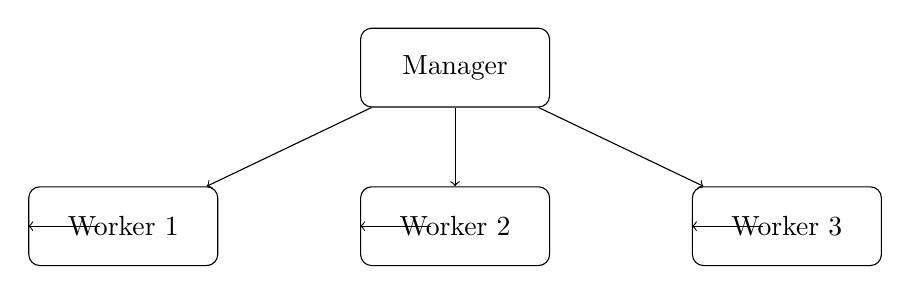
\begin{tikzpicture}[
    node/.style={draw,rounded corners,minimum width=2.4cm,minimum height=1cm},
    yshift=-0.2cm
  ]
    \node[node] (mgr) {Manager};
    \node[node,below left=1cm and 1.8cm of mgr] (w1) {Worker 1};
    \node[node,below=1cm of mgr] (w2) {Worker 2};
    \node[node,below right=1cm and 1.8cm of mgr] (w3) {Worker 3};

    \draw[->] (mgr) -- (w1);
    \draw[->] (mgr) -- (w2);
    \draw[->] (mgr) -- (w3);
    \draw[<-] (w1) -- ++(-0.3,0);
    \draw[<-] (w2) -- ++(-0.3,0);
    \draw[<-] (w3) -- ++(-0.3,0);
  \end{tikzpicture}
  \caption{Manager-worker BSP pattern for data-parallel operations.}
\end{figure}

% ================================================================
\section{Pros and Cons}

\begin{itemize}[itemsep=0pt]
  \item \textbf{Pros}
    \begin{itemize}[itemsep=0pt]
      \item Simple mental model; reuse single-node code inside each worker.
      \item Scales linearly until network shuffle dominates.
    \end{itemize}
  \item \textbf{Cons}
    \begin{itemize}[itemsep=0pt]
      \item Manager may become a bottleneck for large partials (e.g., holistic aggs).
      \item Data skew can cause load imbalance across shards.
    \end{itemize}
\end{itemize}

% ================================================================
\section{Future Work}

\begin{itemize}[itemsep=0pt]
  \item Adaptive shard sizing based on runtime load.
  \item Hierarchical aggregation to relieve manager memory pressure.
  \item Automatic selection of approximate or exact algorithms depending on query SLAs.
\end{itemize}

% ================================================================
\section*{Conclusion}

Non-dedup projection, simple and group-by aggregates, and matrix sums cover a wide swath of data science workloads.  All fit naturally into a manager-worker BSP framework, but careful attention to caching, replication, and skew handling is essential for high performance at scale.:contentReference[oaicite:7]{index=7}

\end{document}
